% !TeX root = Bericht_main.tex
\subsection{Aufgabe 35}

\subsubsection{Aufgabe 35.1}
\begin{figure}[H]
	\centering
	\captionabove{Discretization = linear}
	\subfigure{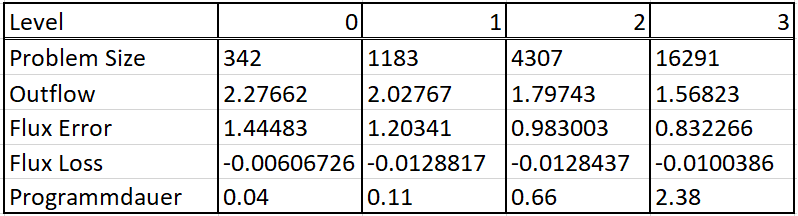
\includegraphics[width=0.99\textwidth]{../Aufgabe35/35_1_linear.png}}	 
\end{figure}

\begin{figure}[H]
	\centering
	\captionabove{Discretization = serendipity}
	\subfigure{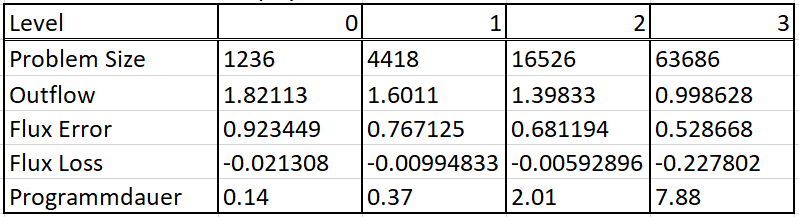
\includegraphics[width=0.99\textwidth]{../Aufgabe35/35_1_serendipity.png}}	 
\end{figure}

\subsubsection{Aufgabe 35.2}
\begin{figure}[H]
	\centering
	\captionabove{symmetric}
	\subfigure{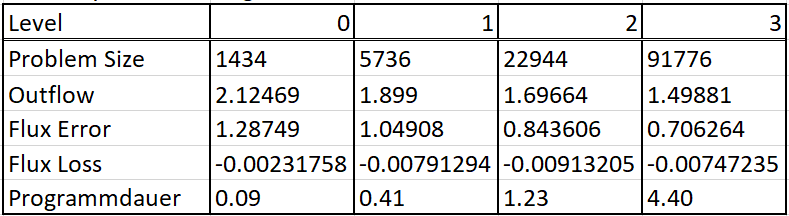
\includegraphics[width=0.99\textwidth]{../Aufgabe35/35_2_sym.png}}	 
\end{figure}

\begin{figure}[H]
	\centering
	\captionabove{non-symmetric}
	\subfigure{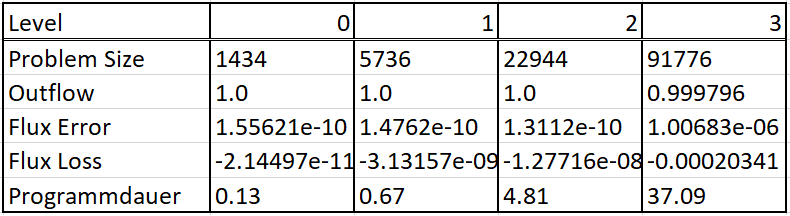
\includegraphics[width=0.99\textwidth]{../Aufgabe35/35_2_nonsym.png}}	 
\end{figure}

\subsubsection{Aufgabe 35.3}
\begin{figure}[H]
	\centering
	\captionabove{deg = 2}
	\subfigure{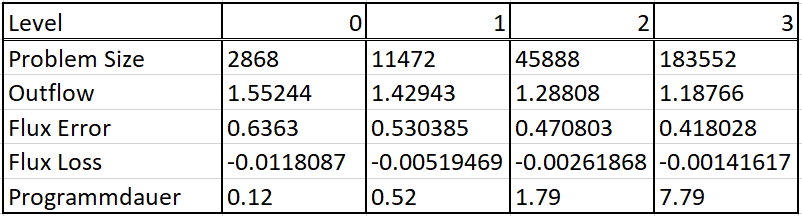
\includegraphics[width=0.99\textwidth]{../Aufgabe35/35_3_level.png}}	 
\end{figure}

\begin{figure}[H]
	\centering
	\captionabove{deg = 2}
	\subfigure{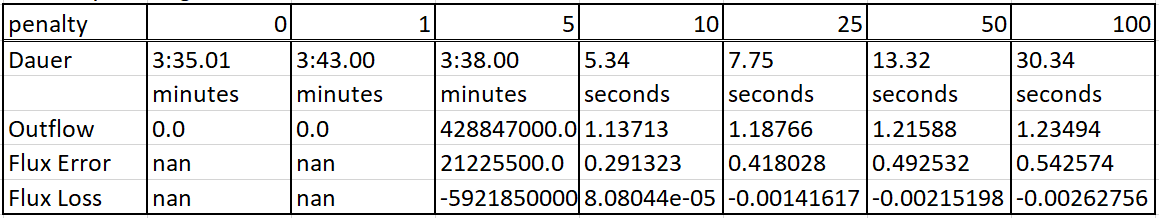
\includegraphics[width=0.99\textwidth]{../Aufgabe35/35_3_dauer.png}}	 
\end{figure}





